\section[La CPU]{La CPU}
\label{sec:cpu}
\sectionframe{images/covers/cover_cpu.jpeg}{La CPU}	 


\subsection[Central Processing Unit]{Central Processing Unit}
\begin{frame}
	\frametitle{Central Processing Unit}
	
%	\begin{block}{Central Processing Unit}
		Una CPU, \textbf{central processing unit} (unità centrale di elaborazione o processore centrale), indica un'unità o sottosistema logico e fisico che sovraintende alle \textbf{funzionalità logiche di elaborazione} principali di un computer.
		La CPU è un'elaborata combinazione di transistor che può essere definita \textit{circuito integrato}.\\~\\
		\pause
		All'interno della CPU individuiamo tre elementi fondamentali:
		\begin{itemize}
			\item \textbf{la CU}, \textit{Control Unit} (l’unità di controllo):\\
			coordina l'esecuzione delle operazioni da parte del processore;
			\item \textbf{la ALU}, \textit{Arithmetic-Logic Unit} (l’Unità Aritmetico-Logica):\\
			si occupa di eseguire le operazioni aritmetico-logiche;
			\item \textbf{i registri di memoria}:\\
			diverse \textit{celle di memoria} dedicate a scopi specifici che vengono utilizzati per il controllo dell'esecuzione di un programma.
		\end{itemize}
%	\end{block}
	
\end{frame}



\begin{frame}
%	\frametitle{L'architettura di un computer}
	
	\begin{figure}[!htbp] 
		\centering
		%\advance\leftskip-0.25cm
		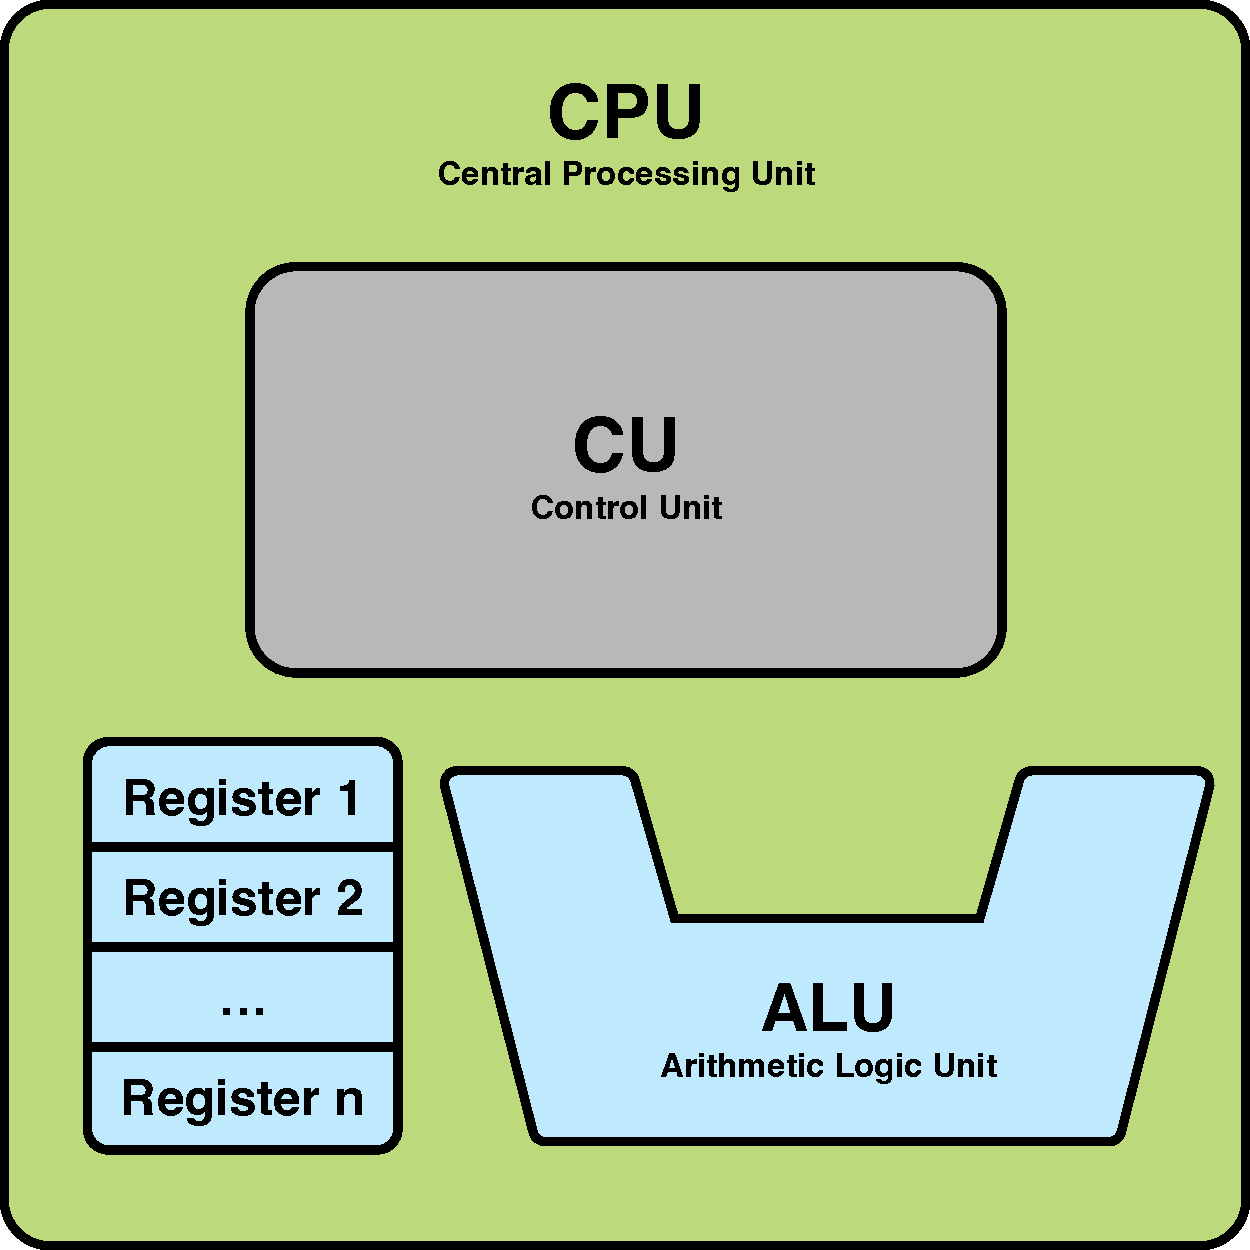
\includegraphics[width=0.58\linewidth]{images/4_cpu/architecture_cpu_simple.pdf}
		\caption{La CPU: CU, ALU e registri}
		\label{fig:cpu_simple}
	\end{figure}
	 
\end{frame}




\subsection[Il ciclo di macchina]{Il ciclo di macchina}

\begin{frame}
	\frametitle{Il ciclo di macchina}
	
	\begin{block}{Il ciclo di macchina}
		 La CPU esegue le istruzioni macchina in maniera ciclica.\\
		 Il cosiddetto \textbf{ciclo di macchina} può essere idealmente suddiviso in 4 parti:
		 
		\begin{columns}			
			\column{0.65\linewidth}
			\begin{enumerate}
			 	\item {\color{CpuGreen}\textbf{fetch}}: prelevamento dalla memoria del codice macchina dell’istruzione da eseguire;
			 	\item {\color{CpuRed}\textbf{decode}}: l'istruzione prelevata viene trasferita in un registro specifico e quindi codificata (tradotta);
			 	\item {\color{CpuBlue}\textbf{fetch operands}}: se necessario si prelevano anche gli operandi necessari all'istruzione;
			 	\item {\color{CpuYellow}\textbf{execute}}: la CPU quindi emette i segnali necessari all'esecuzione dell’istruzione.
			 \end{enumerate}
			
			\column{0.35\linewidth}
			\begin{figure}[!htbp]
				\centering 
				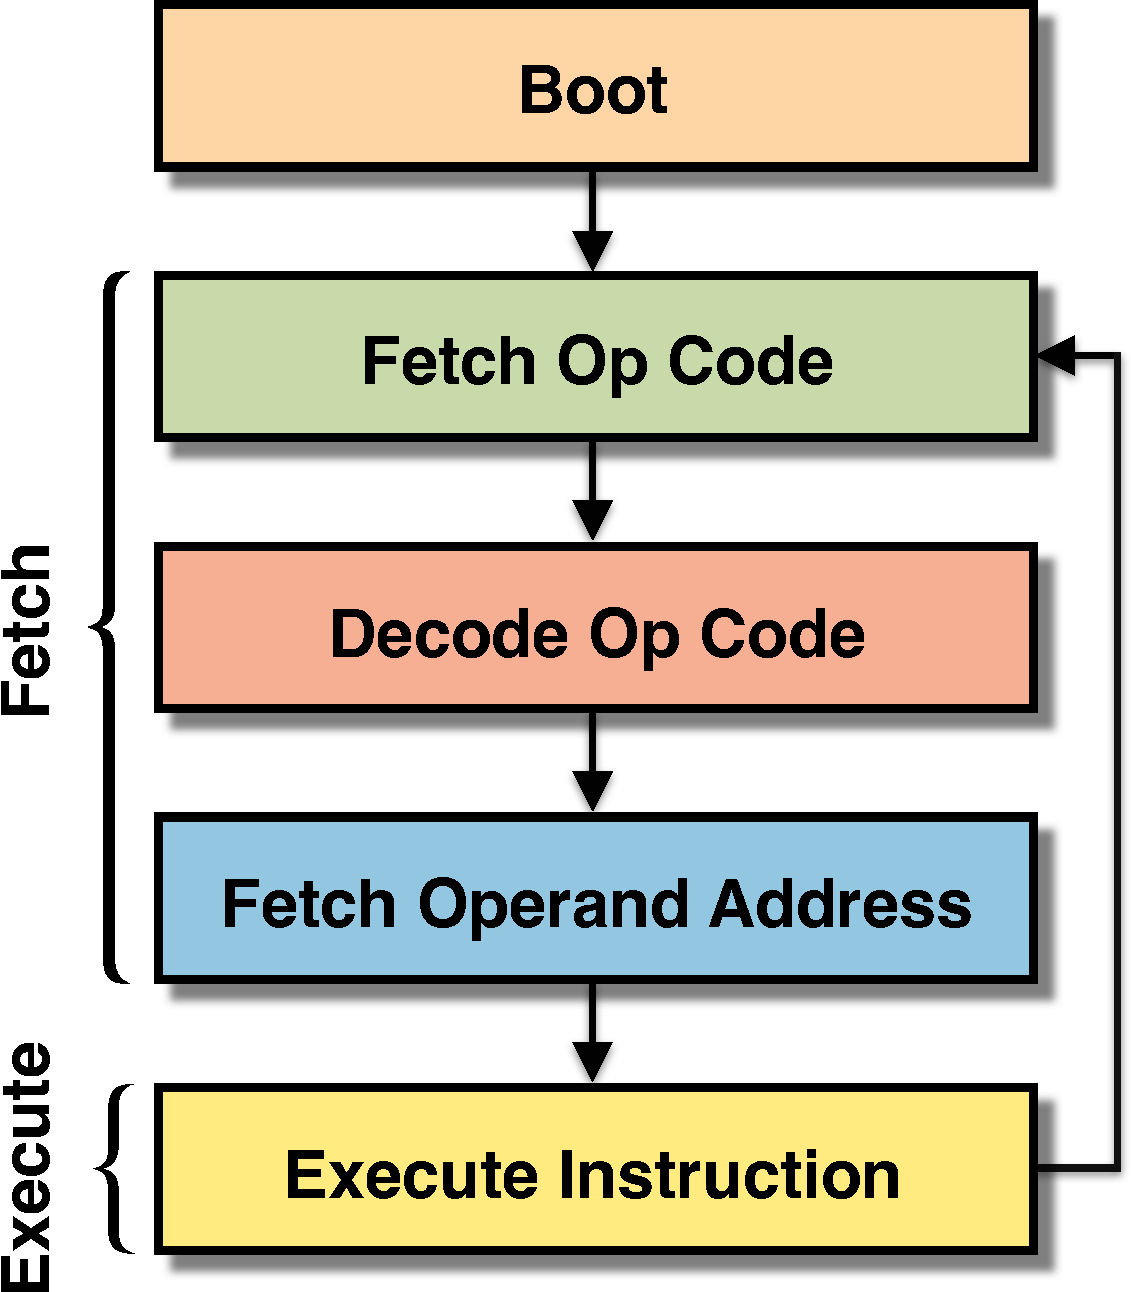
\includegraphics[width=0.95\linewidth]{images/4_cpu/architecture_cpu_cycle.pdf}
%				\caption{}
			\end{figure} 
		\end{columns}
		 
		 
	\end{block}
	
\end{frame}


\begin{frame}
	\frametitle{Il ciclo di macchina: schema della CPU} % ($\bigstar$)
	
	\begin{figure}[!htbp] 
		\centering
		%\advance\leftskip-0.25cm
		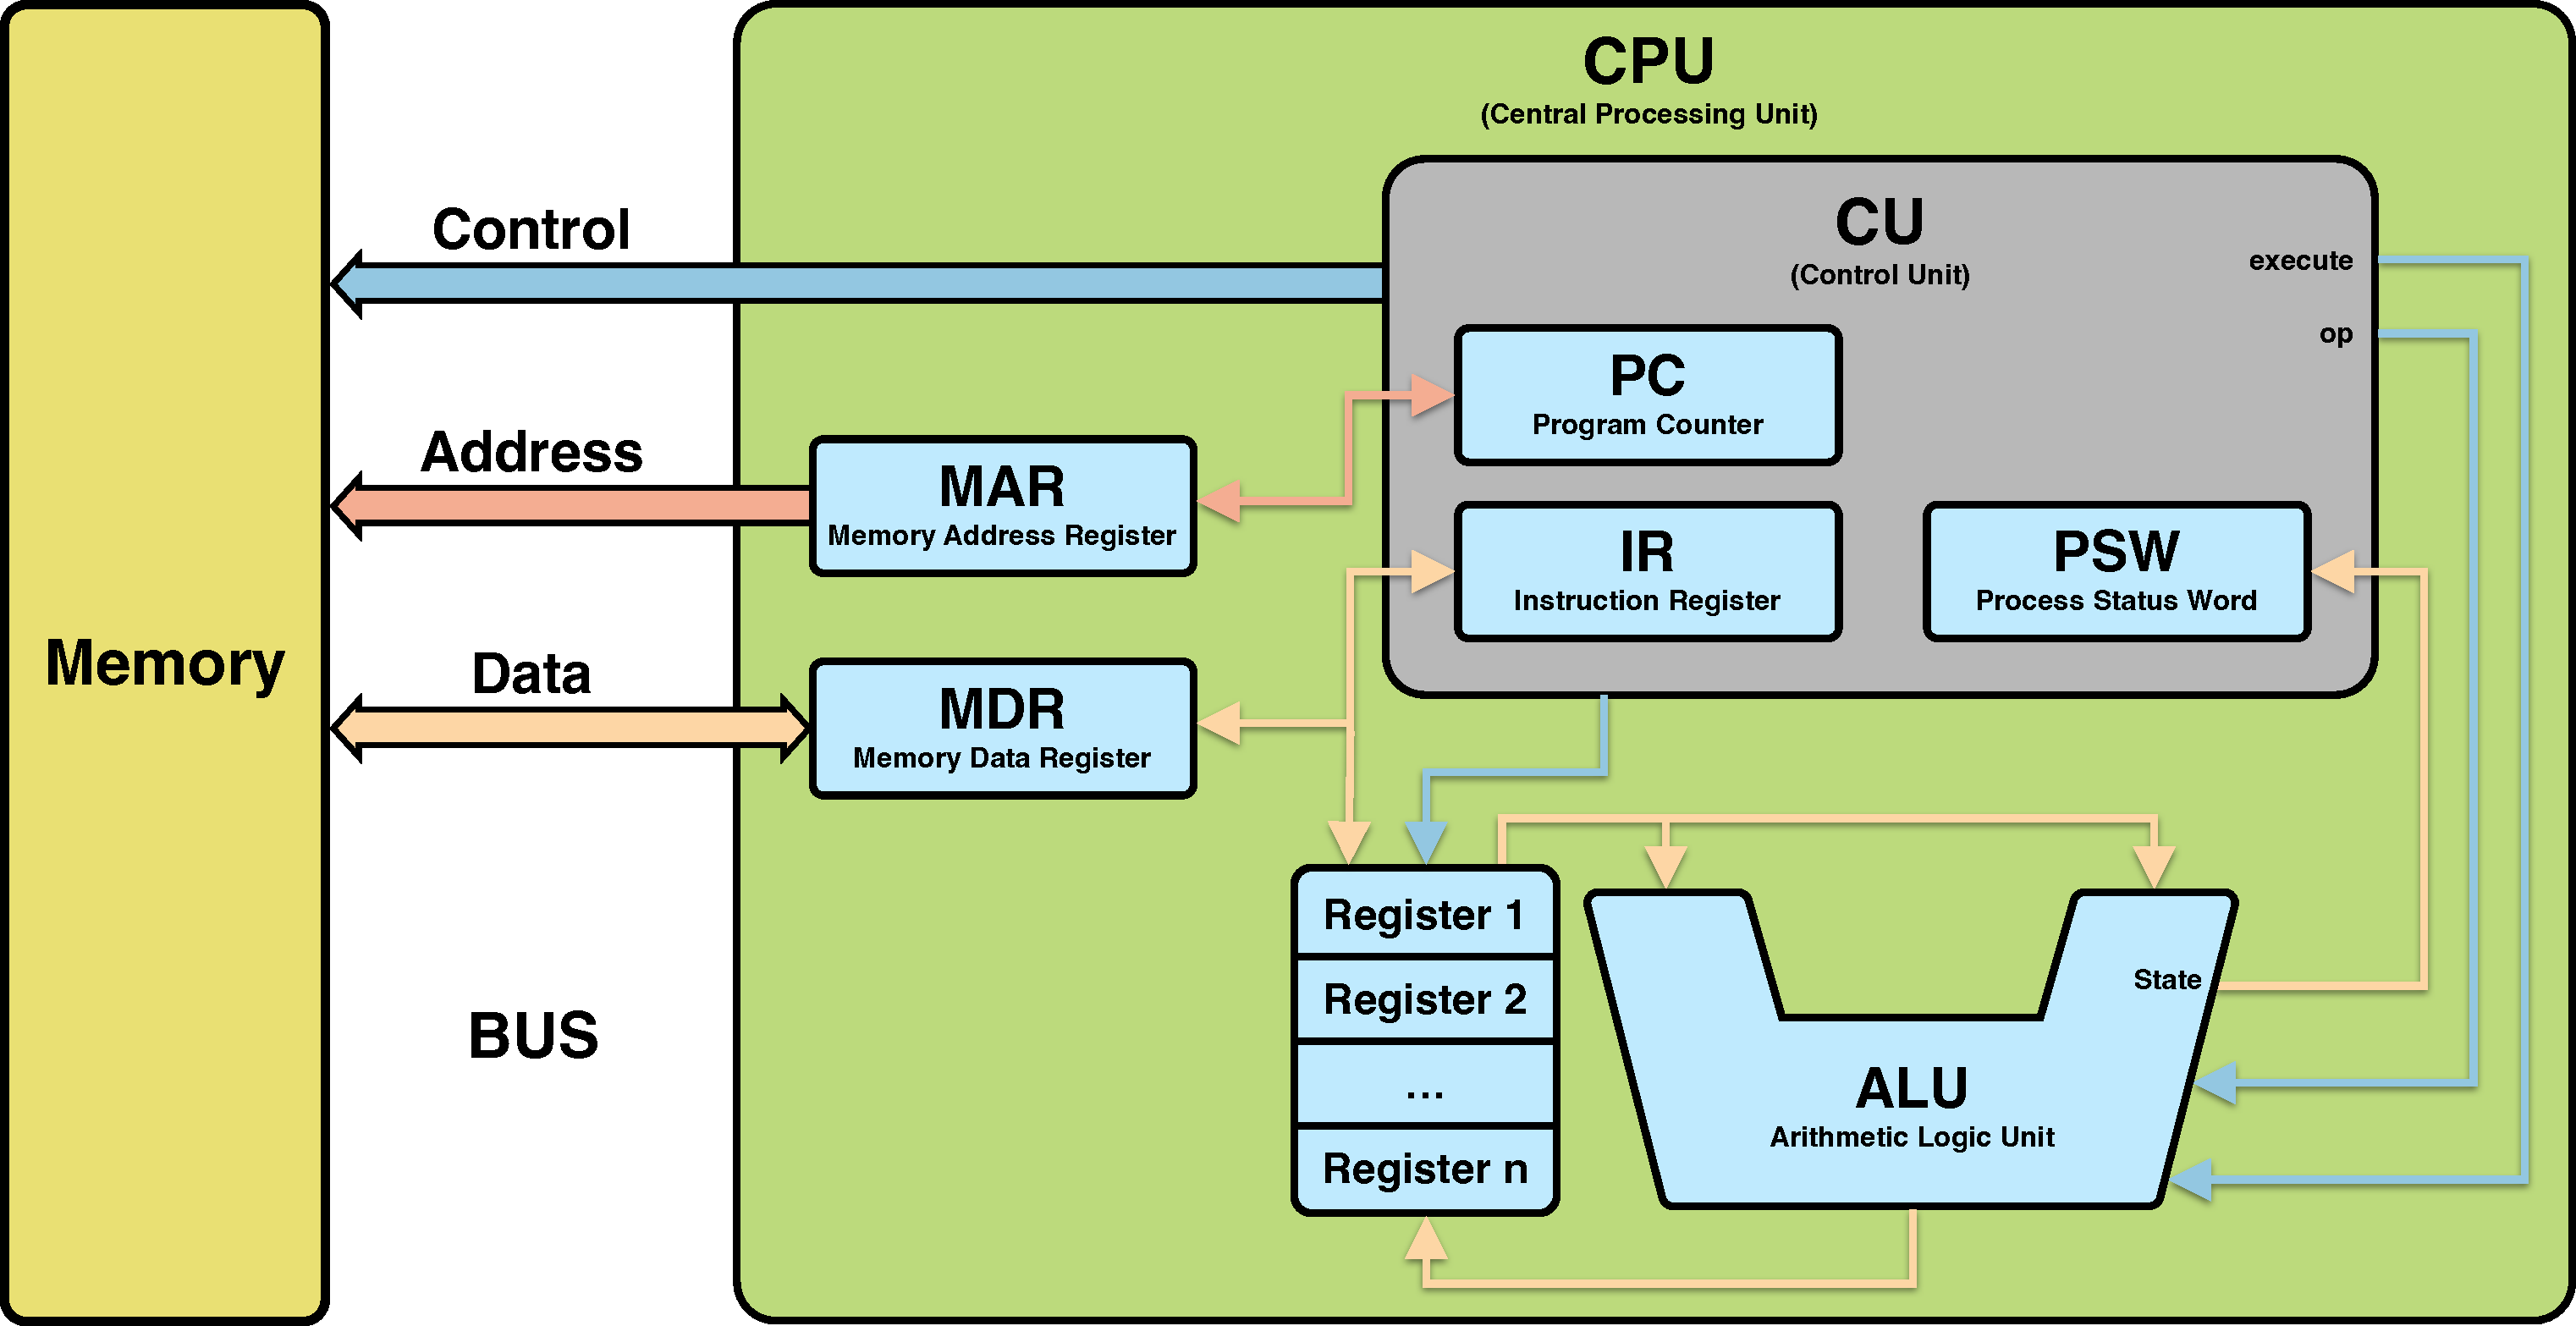
\includegraphics[width=1.0\linewidth]{images/4_cpu/architecture_cpu_complex.pdf}
%		\caption{La CPU: CU, ALU e registri}
		\label{fig:cpu_complex}
	\end{figure}
	 
\end{frame}


\begin{frame}
	\frametitle{Il ciclo di macchina: schema della CPU}
	
	\underline{Registri non accessibili al programmatore}:
	\begin{itemize}
		\item il \textbf{MAR}, \textit{Memory Address Register}: è un registro interno collegato direttamente al BUS indirizzi. Contiene gli indirizzi necessari alla selezione della cella di memoria oppure al dispositivo di I/O;
		\item il \textbf{MDR}, \textit{Memory Data Register}: è un registro interno collegato direttamente al BUS dati. Contiene i dati che la CPU vuole inviare o ricevere dalla memoria o dai dispositivi di I/O;% Il registro MDR è una sorta di memoria di transito.
		\item l'\textbf{IR}, \textit{Instruction Register}: è il registro che contiene l'istruzione che sta per essere eseguita;
	\end{itemize}
	
	\underline{Registri accessibili al programmatore}:
	\begin{itemize}
		\item il \textbf{PC}, \textit{Program Counter}: è il registro che contiene l'indirizzo di memoria della prossima istruzione da eseguire;
		\item il \textbf{PSW}, \textit{Process Status Word}: anche detto \textit{Flag Register}
	\end{itemize}
	 
\end{frame}


\begin{frame}
	\frametitle{Il ciclo di macchina: il Flag Register}
	
	\begin{figure}[!htbp] 
		\centering
		%\advance\leftskip-0.25cm
		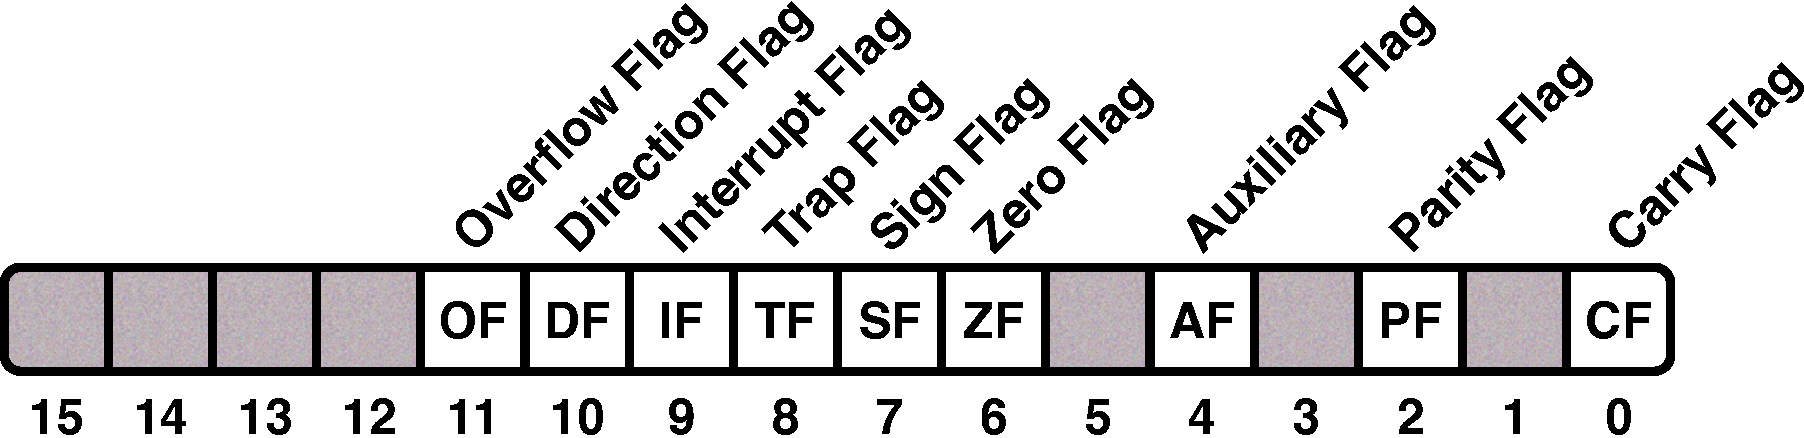
\includegraphics[width=0.7\linewidth]{images/4_cpu/flag_register.pdf}
%		\caption{}
		\label{fig:cpu_complex}
	\end{figure}
	
	Il \textbf{Flag Register} (PSW, Process Status Word) è l'unico registro il cui contenuto non ha un significato nel suo complesso, ma \textbf{ciascun bit} che lo compone \textbf{ha un suo significato specifico}.\\
	\underline{L’ALU, a ogni operazione aritmetico-logica ne aggiorna il contenuto}.\\~\\
	Le informazioni contenute in questo registro sono essenziali per la costruzione degli algoritmi dei programmi. Controllando il valore dei flag possiamo infatti realizzare le strutture fondamentali della programmazione (condizione, iterazione, sottoprogrammi).
	 
\end{frame}


\begin{frame}
	\frametitle{Il ciclo di macchina: il Flag Register}
	
	\begin{figure}[!htbp] 
		\centering
		%\advance\leftskip-0.25cm
		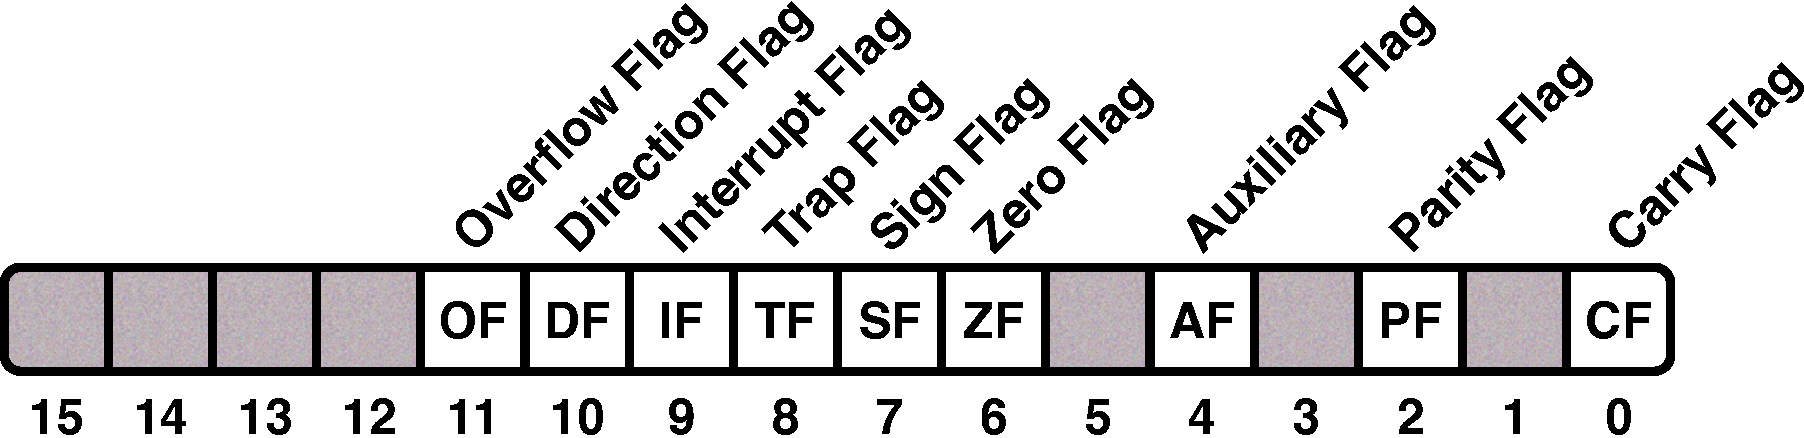
\includegraphics[width=0.7\linewidth]{images/4_cpu/flag_register.pdf}
%		\caption{}
		\label{fig:cpu_complex}
	\end{figure}
	
%	\begin{itemize}
%		\item il bit OF (Overflow Flag) vale 1 se il segno del risultato dell’ultima operazione aritmetico-logica discorda dal segno degli operandi
%		\item il bit SF (Sign Flag) vale 1 se  il risultato dell’ultima operazione aritmetico-logica è negativo
%		\item il bit ZF (Zero Flag) vale 1 se il risultato dell’ultima istruzione aritmetico-logica è zero
%		\item il bit PF (Parity Flag) vale 1 se nel risultato dell’ultima operazione aritmetico-logica il numero di bit a 1 del risultato è pari
%		\item il bit CF (Carry Flag) vale 1 se l’ultima istruzione aritmetico-logica aveva un riporto
%	\end{itemize}

	Tutti i flag si riferiscono all'ultima operazione aritmetico-logica:
	\begin{itemize}
		\item il bit CF (Carry Flag) vale 1 se si è avuto un riporto
		\item il bit PF (Parity Flag) vale 1 se nel risultato il numero di bit a 1 del risultato è pari
		\item il bit ZF (Zero Flag) vale 1 se il risultato è zero
		\item il bit SF (Sign Flag) vale 1 se  il risultato è negativo
		\item il bit OF (Overflow Flag) vale 1 se il segno del risultato discorda dal segno degli operandi
	\end{itemize}	 
\end{frame}



\subsubsection[Fetch]{Fetch}
\begin{frame}
	\frametitle{{\color{GradientDescentDiagramGreen}Hierarchical Clustering}}
	\frametitle{Il ciclo di macchina: il {\color{CpuGreen}\textbf{fetch}}}
	
	\begin{block}{Il ciclo di macchina: il fetch}
		\begin{enumerate}
			\item la CPU mette il valore di PC (indirizzo della prossima istruzione da leggere dalla memoria) su MAR e attiva la linea Leggi (Control BUS);
			\item la memoria attraverso il BUS indirizzi accede a MAR e, una volta reperito quanto richiesto, lo scrive su MDR attraverso il BUS dati;
		\end{enumerate}
	\end{block}
	
	\begin{figure}[!htbp] 
		\centering
		%\advance\leftskip-0.25cm
		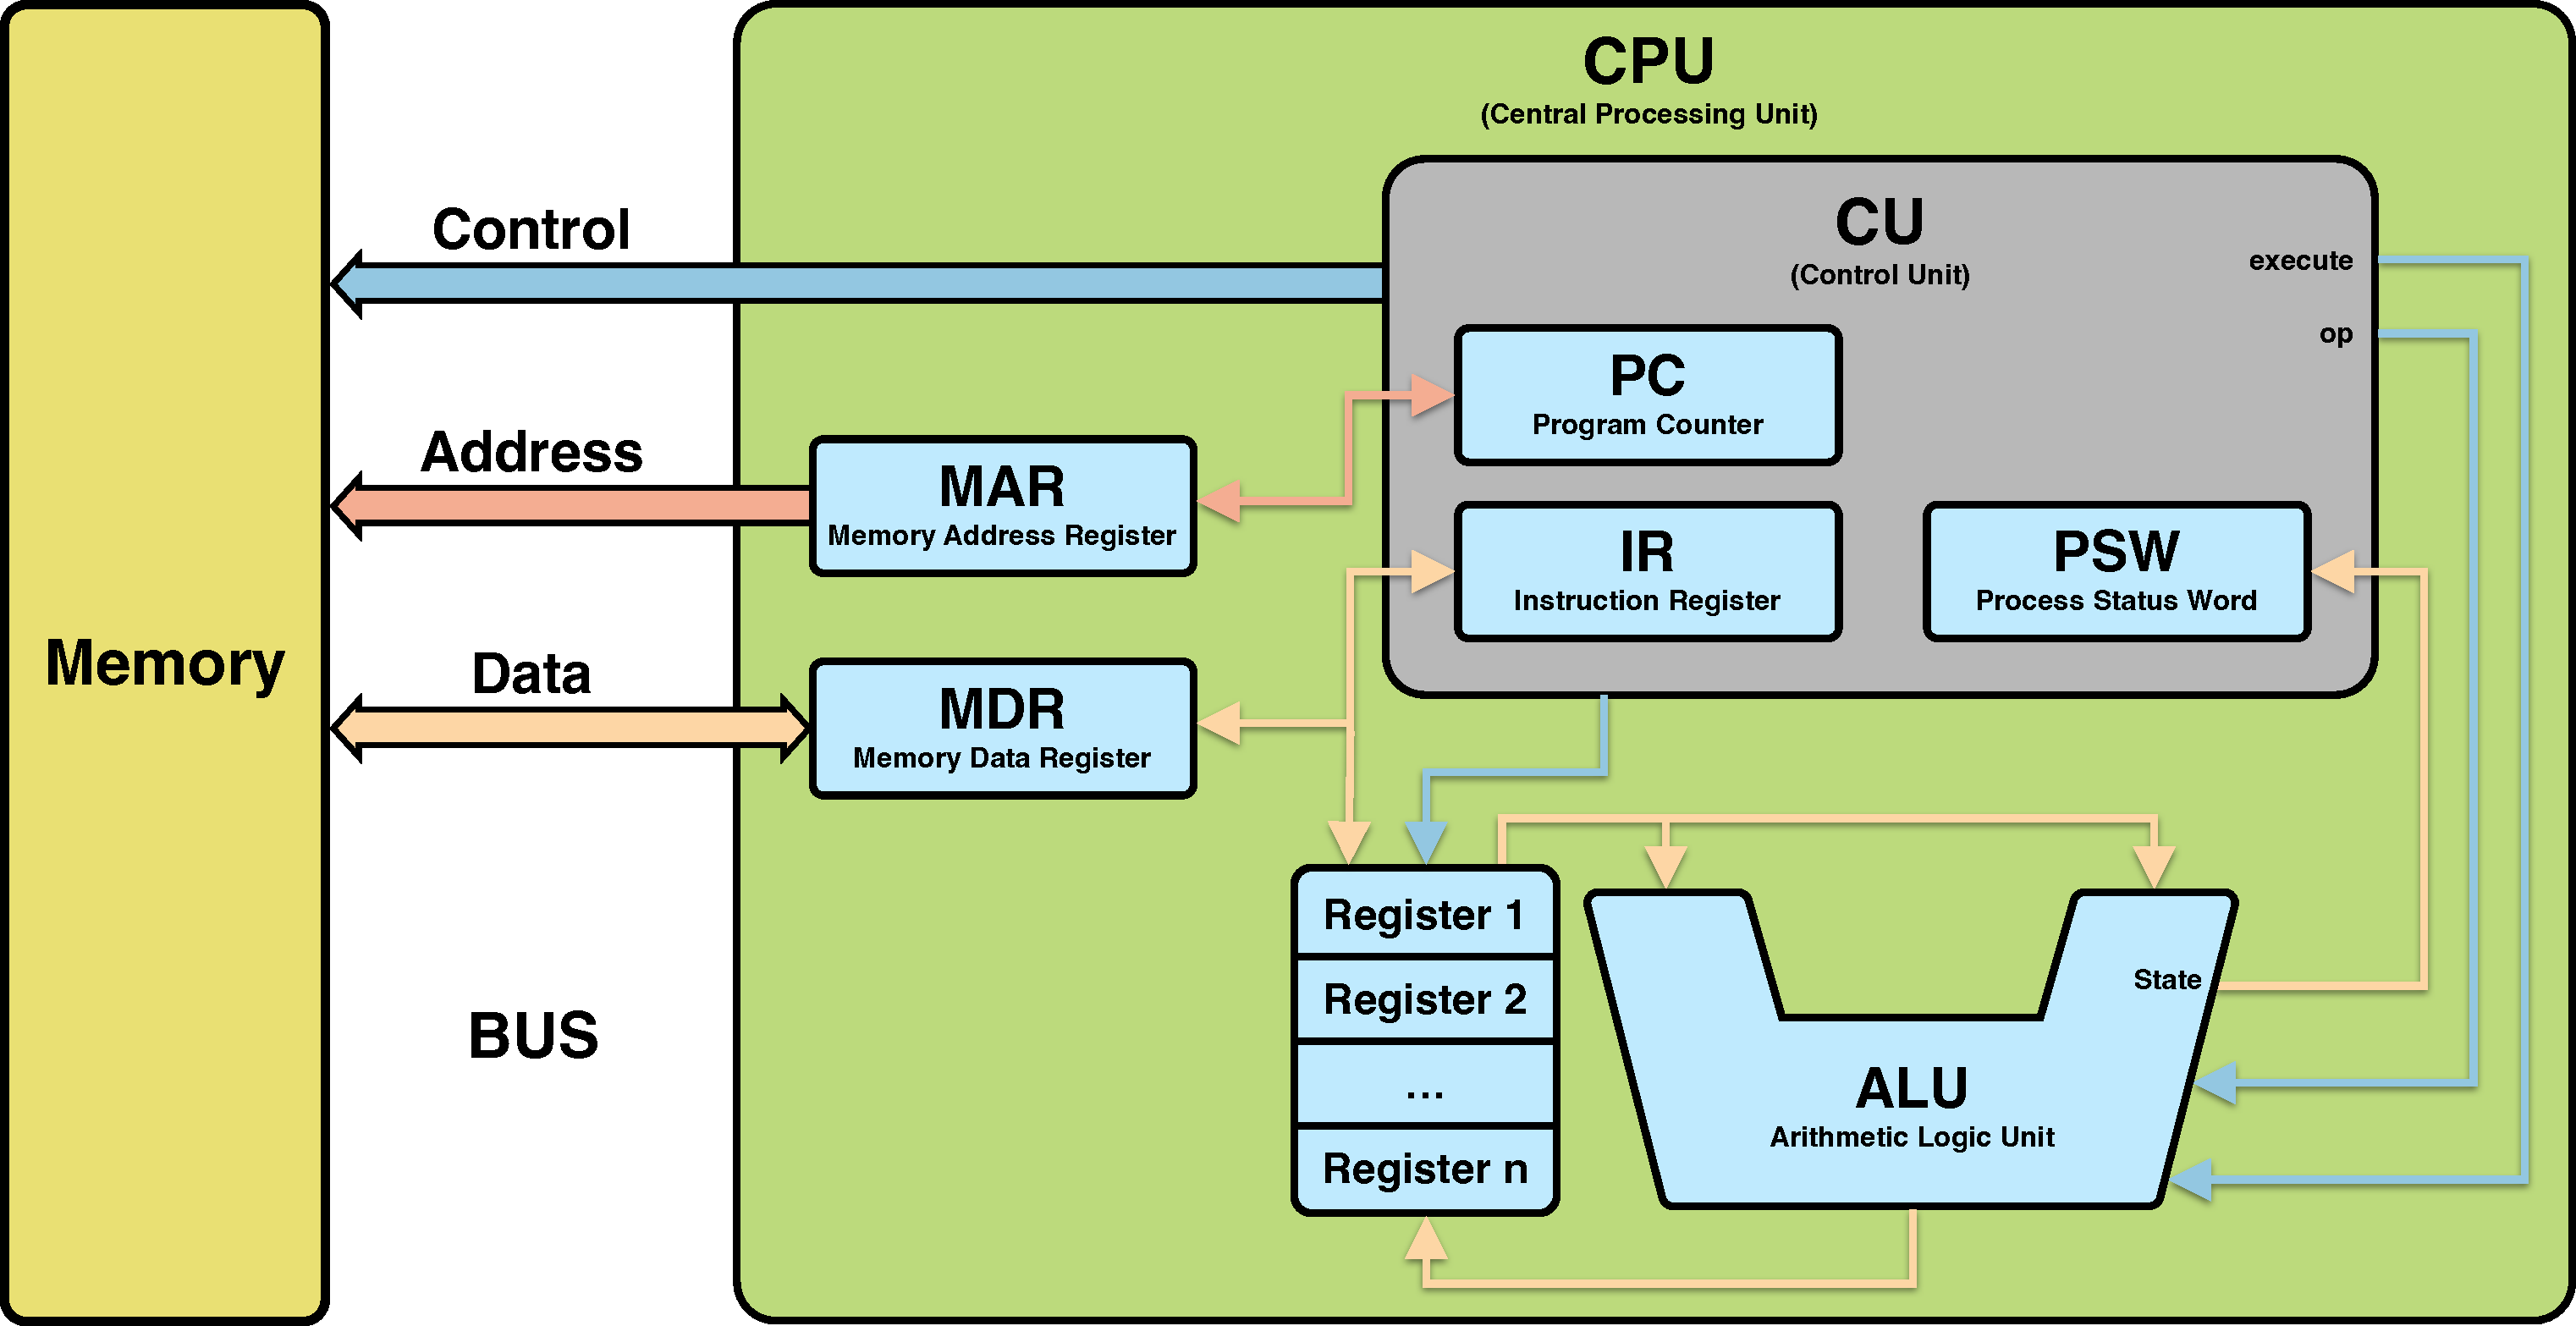
\includegraphics[width=0.7\linewidth]{images/4_cpu/architecture_cpu_complex.pdf}
%		\caption{La CPU: CU, ALU e registri}
		\label{fig:cpu_complex}
	\end{figure}
	
\end{frame}


\subsubsection[Decode]{Decode}
\begin{frame}
	\frametitle{Il ciclo di macchina: il {\color{CpuRed}\textbf{decode}}}
	
	\begin{block}{Il ciclo di macchina: il decode}	
	
		\begin{enumerate}
			\setcounter{enumi}{2}
			\item la CPU copia su IR il valore di MDR e decodifica l'istruzione;
			\item l'istruzione passa in esecuzione sulla ALU;
		\end{enumerate}
	
	\end{block}
	
	\begin{figure}[!htbp] 
		\centering
		%\advance\leftskip-0.25cm
		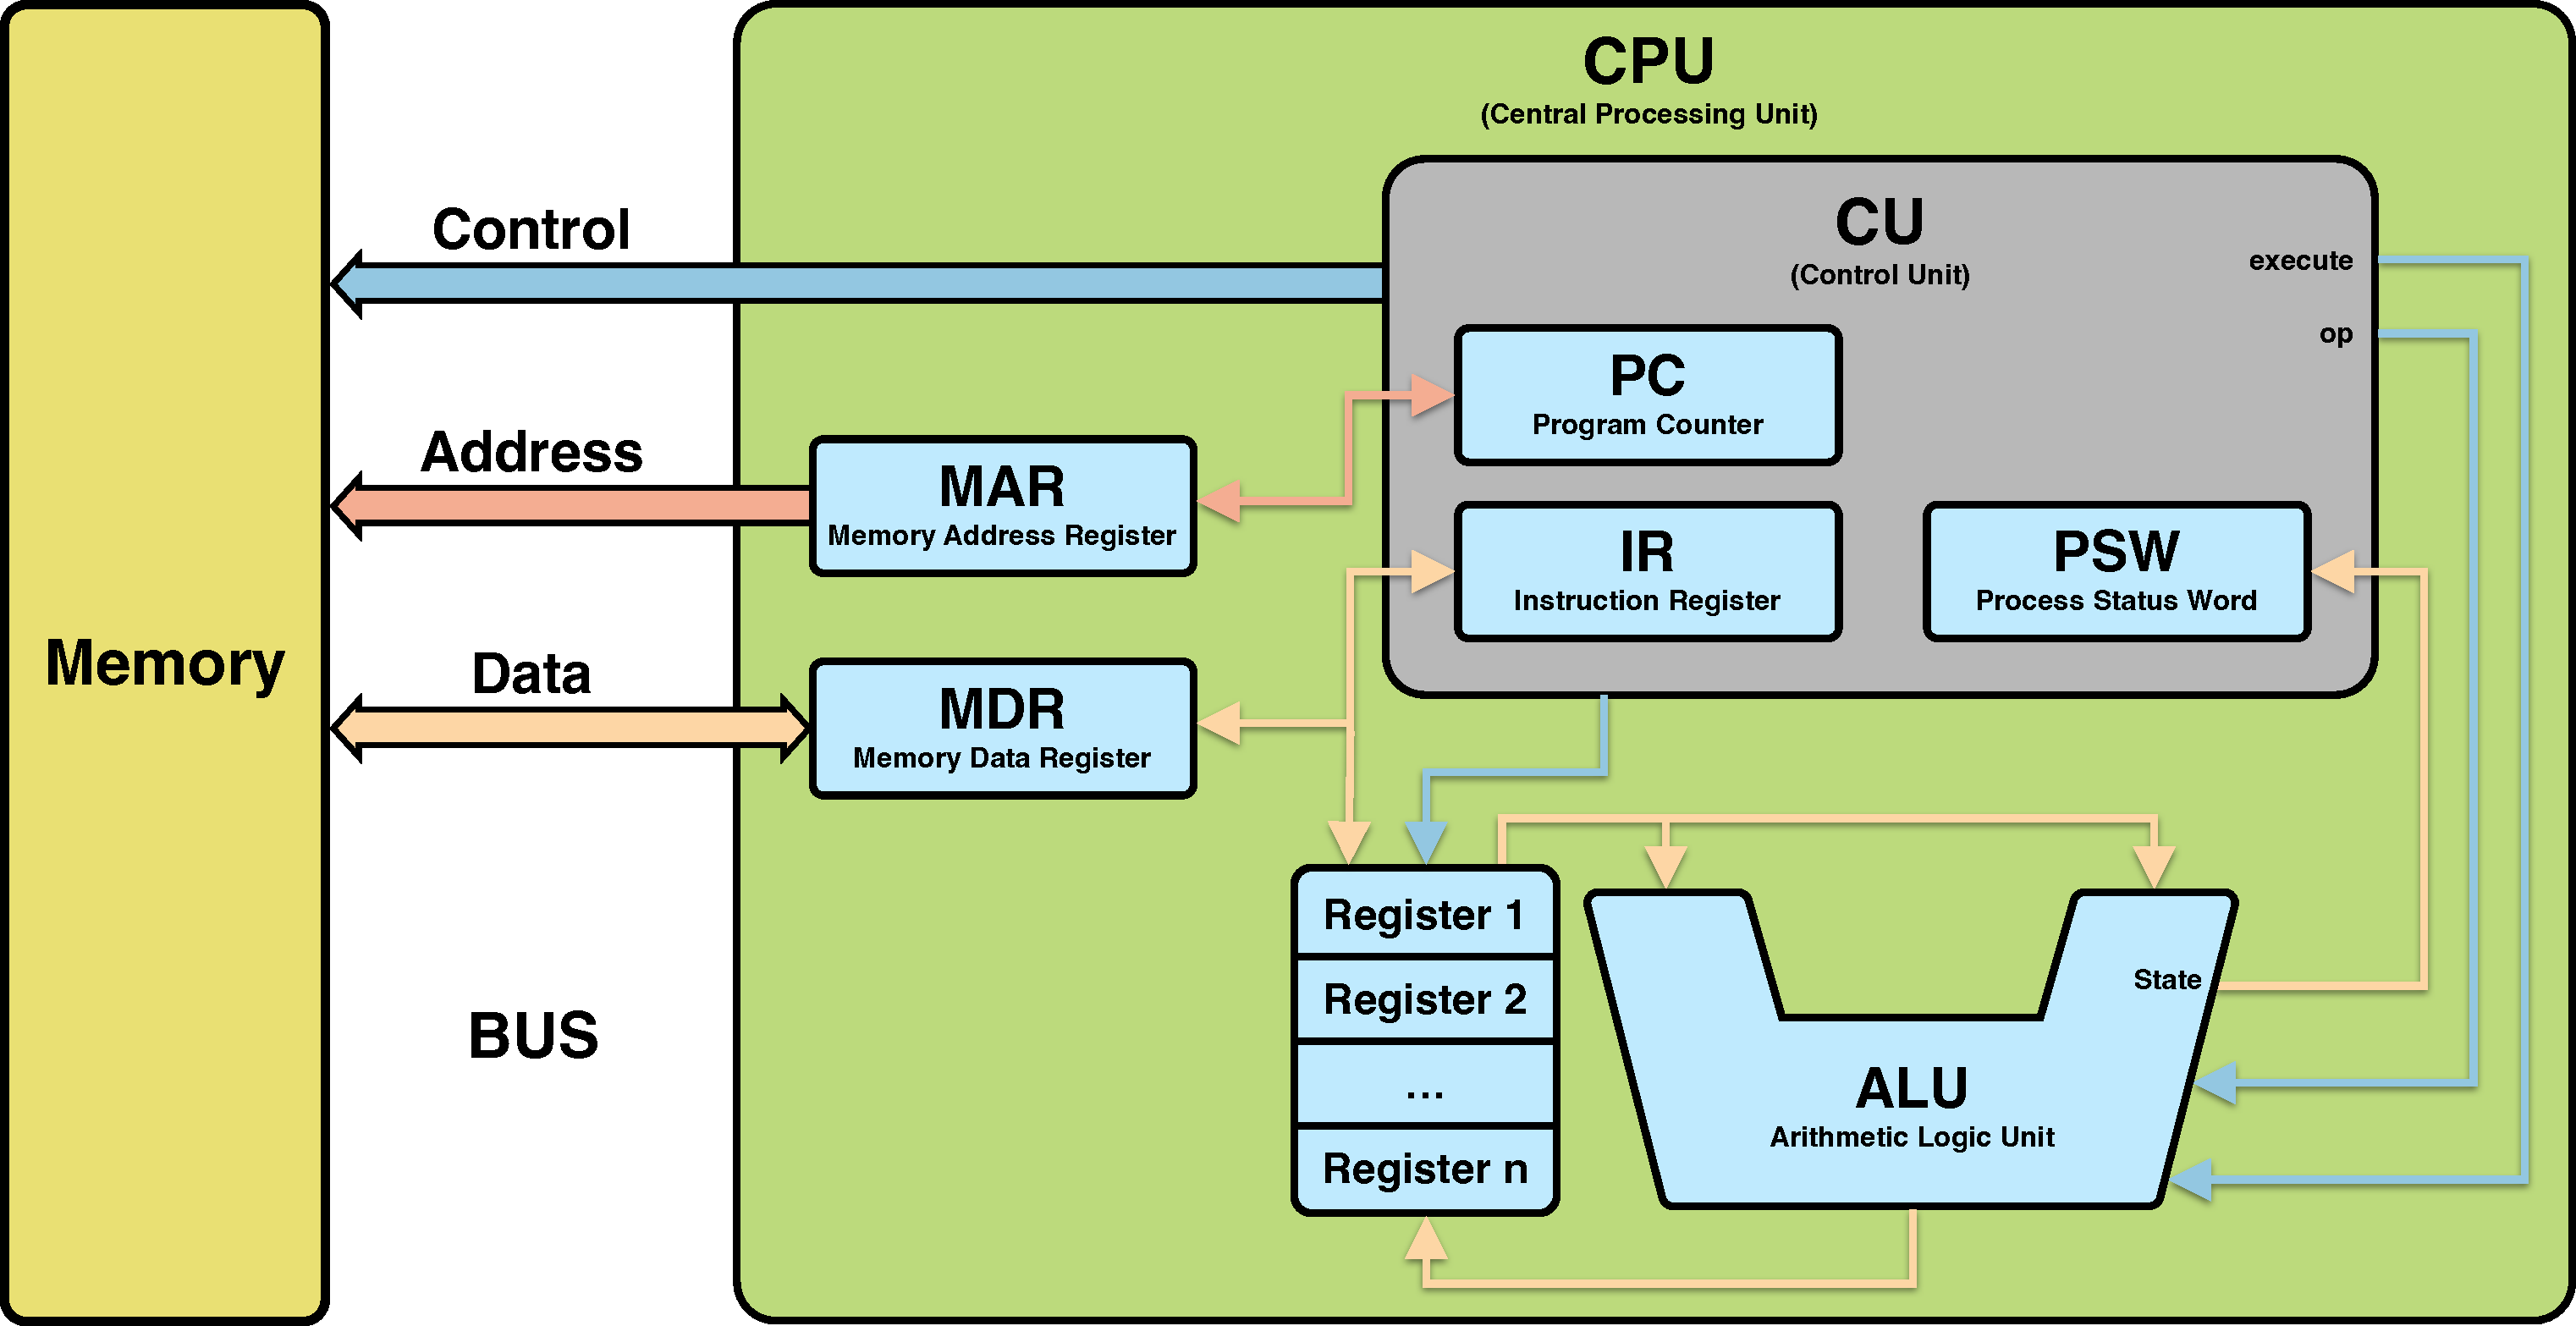
\includegraphics[width=0.7\linewidth]{images/4_cpu/architecture_cpu_complex.pdf}
%		\caption{La CPU: CU, ALU e registri}
		\label{fig:cpu_complex}
	\end{figure}
	
\end{frame}

\subsubsection[Fetch Operands]{Fetch Operands}
\begin{frame}
	\frametitle{Il ciclo di macchina: il {\color{CpuBlue}\textbf{fetch degli operandi}}}
	
	\begin{block}{Il ciclo di macchina: il fetch degli operandi}
		\begin{enumerate}
			\setcounter{enumi}{4}
			\item se l'istruzione prevede la lettura di operandi dalla memoria, questi devono essere caricati sui registri; per ciascun operando da reperire: 
				\begin{enumerate}
					\item la CPU mette l'indirizzo dell'operando su MAR e attiva la linea Leggi;
					\item la memoria attraverso il BUS indirizzi accede a MAR e, una volta reperito quanto richiesto, lo scrive su MDR attraverso il BUS dati;
					\item la CPU copia sul registro destinazione il valore dell'operando che è in MDR;
				\end{enumerate}
			
		\end{enumerate}
	
	\end{block}
	
	\begin{figure}[!htbp] 
		\centering
		%\advance\leftskip-0.25cm
		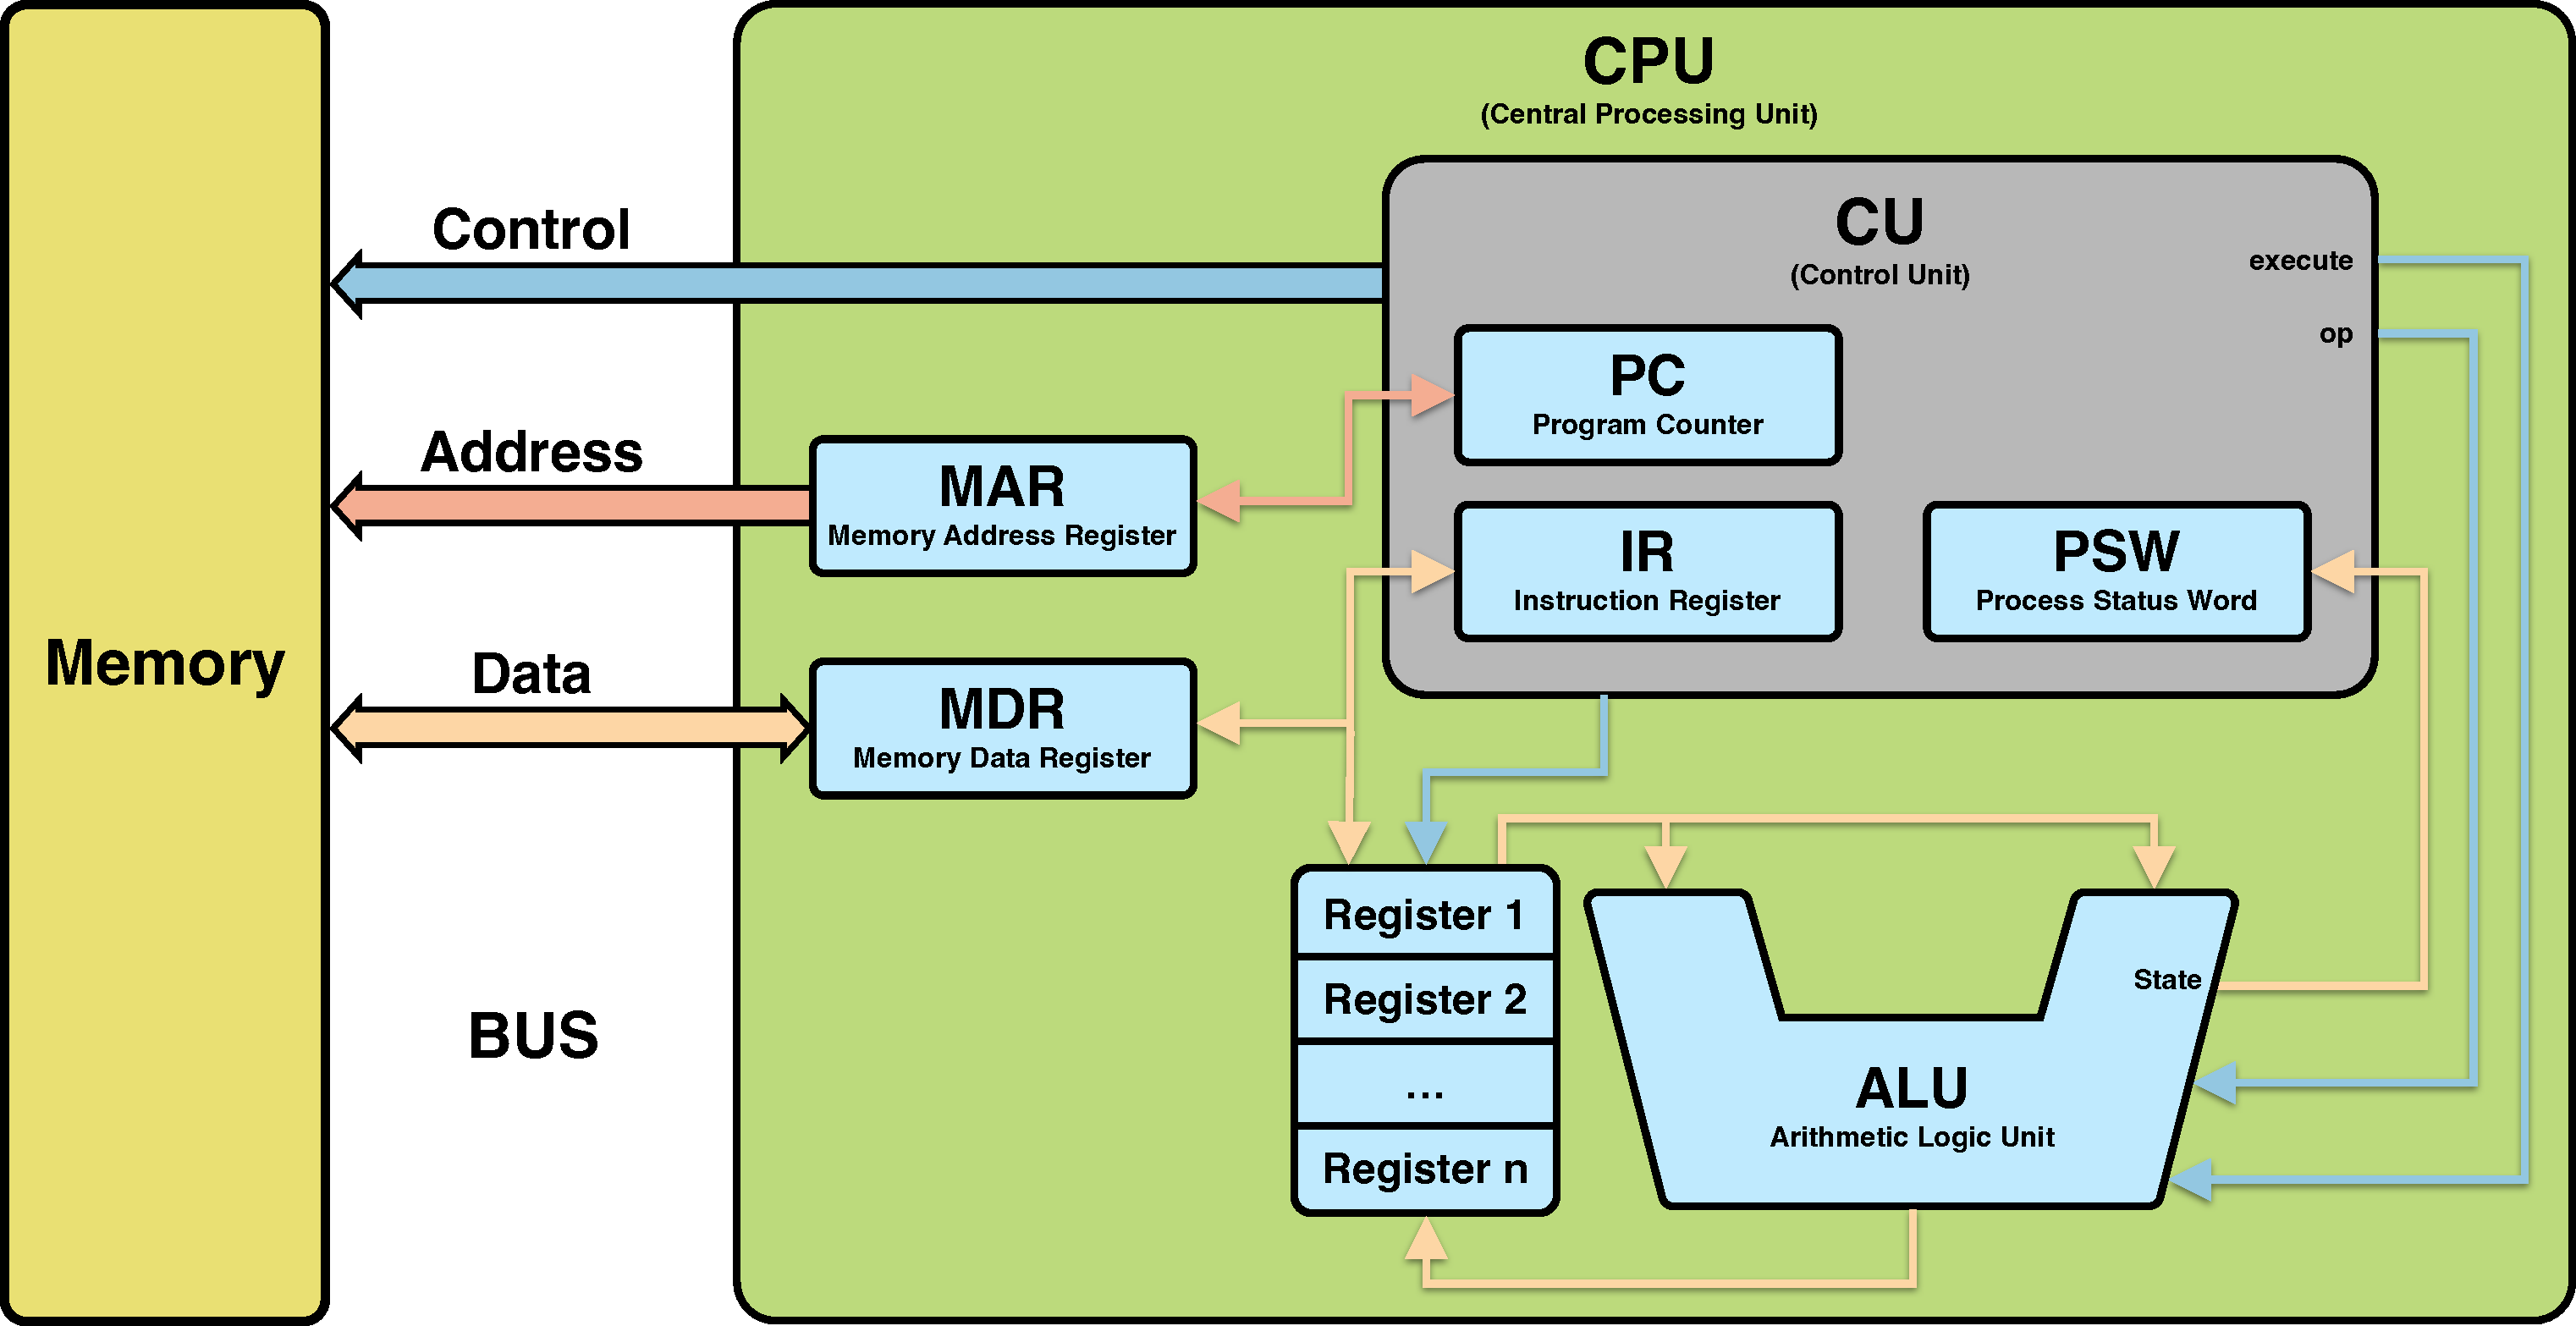
\includegraphics[width=0.51\linewidth]{images/4_cpu/architecture_cpu_complex.pdf}
%		\caption{La CPU: CU, ALU e registri}
		\label{fig:cpu_complex}
	\end{figure}
	
\end{frame}


\subsubsection[Execute]{Execute}
\begin{frame}
	\frametitle{Il ciclo di macchina: l'{\color{CpuYellow}\textbf{execute}}}
	
	\begin{block}{Il ciclo di macchina: l'execute}	
		\begin{enumerate}
			\setcounter{enumi}{5}
			\item terminata l'esecuzione la CPU copia sul registro destinazione il valore prodotto dalla ALU; se è prevista scrittura in memoria del risultato:
				
				\begin{enumerate}
					\item la CPU mette l'indirizzo della cella di destinazione su MAR e il risultato su MDR e attiva la linea Scrivi (Control BUS);
					\item la memoria attraverso il BUS indirizzi accede a MAR, attraverso il BUS dati a MDR e, una volta reperito il valore in MDR, lo scrive sulla propria cella interna indicata da MAR;
				\end{enumerate}
		\end{enumerate}
	
	\end{block}
	
	\begin{figure}[!htbp] 
		\centering
		%\advance\leftskip-0.25cm
		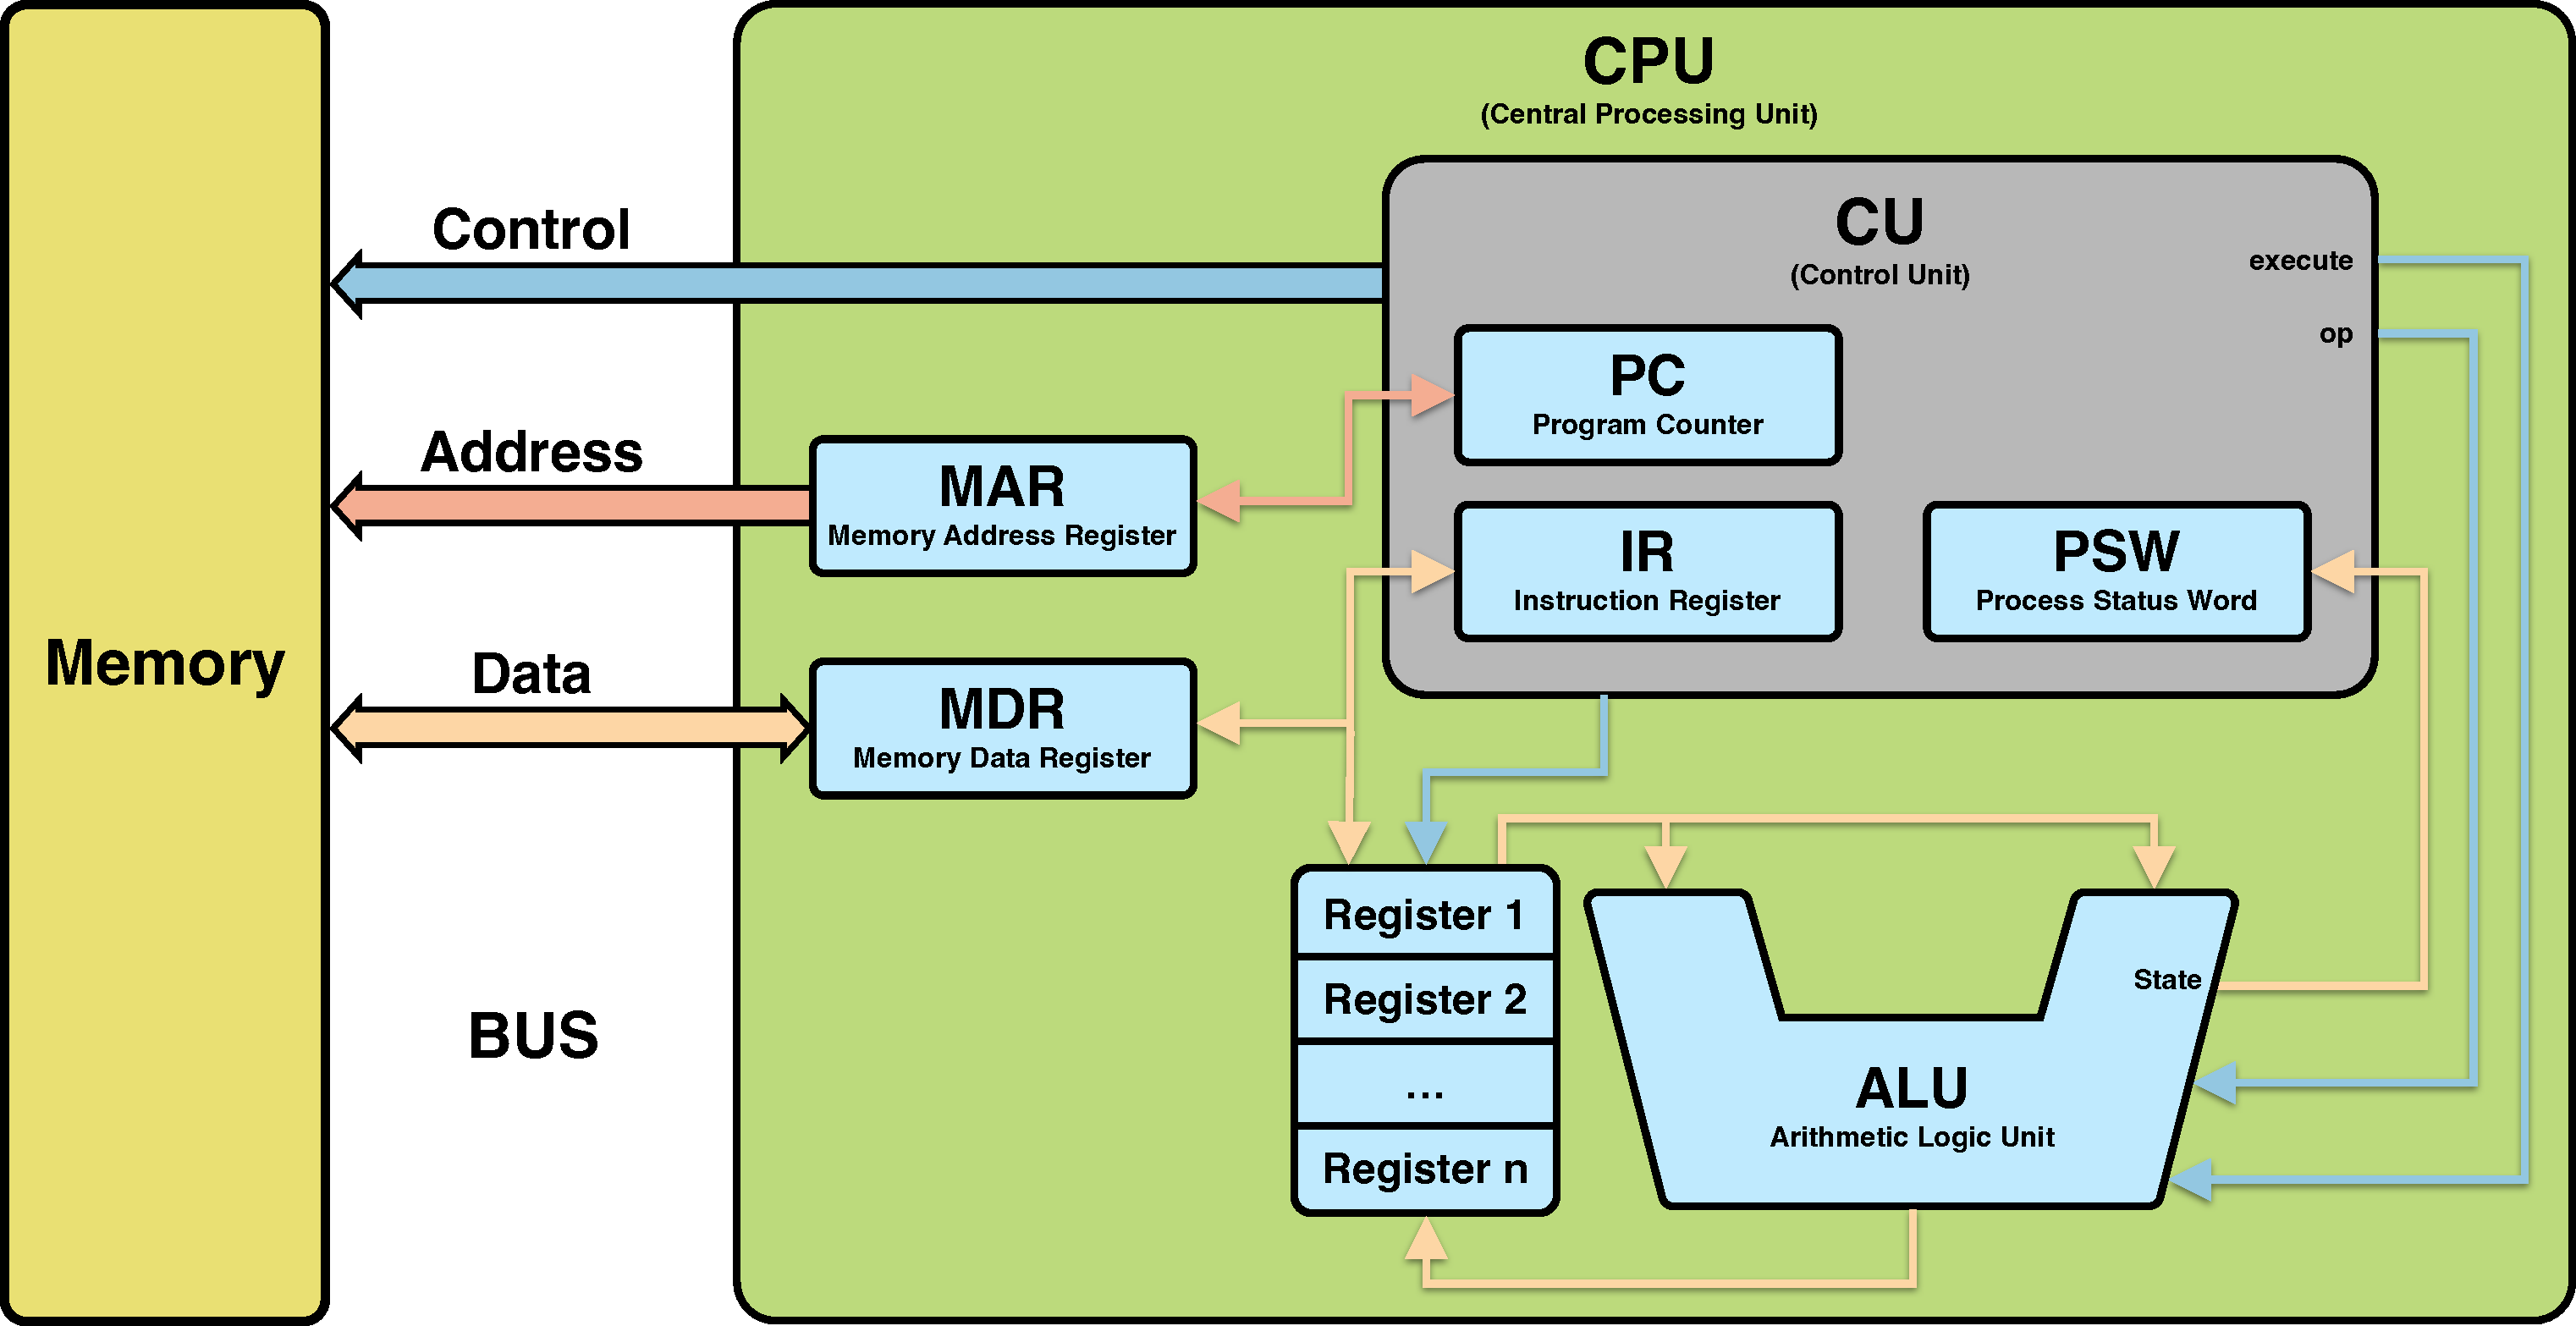
\includegraphics[width=0.51\linewidth]{images/4_cpu/architecture_cpu_complex.pdf}
%		\caption{La CPU: CU, ALU e registri}
		\label{fig:cpu_complex}
	\end{figure}
	
\end{frame}


\begin{frame}
	\frametitle{Il ciclo di macchina: l'{\color{CpuYellow}\textbf{execute}}}
	
	\begin{block}{Il ciclo di macchina: l'execute}	
		\begin{enumerate}
			\setcounter{enumi}{6}
			\item Si ritorna al punto 1 dopo aver aggiornato il valore di PC (prossima istruzione da eseguire).
		\end{enumerate}
	
	\end{block}
	
	\begin{figure}[!htbp] 
		\centering
		%\advance\leftskip-0.25cm
		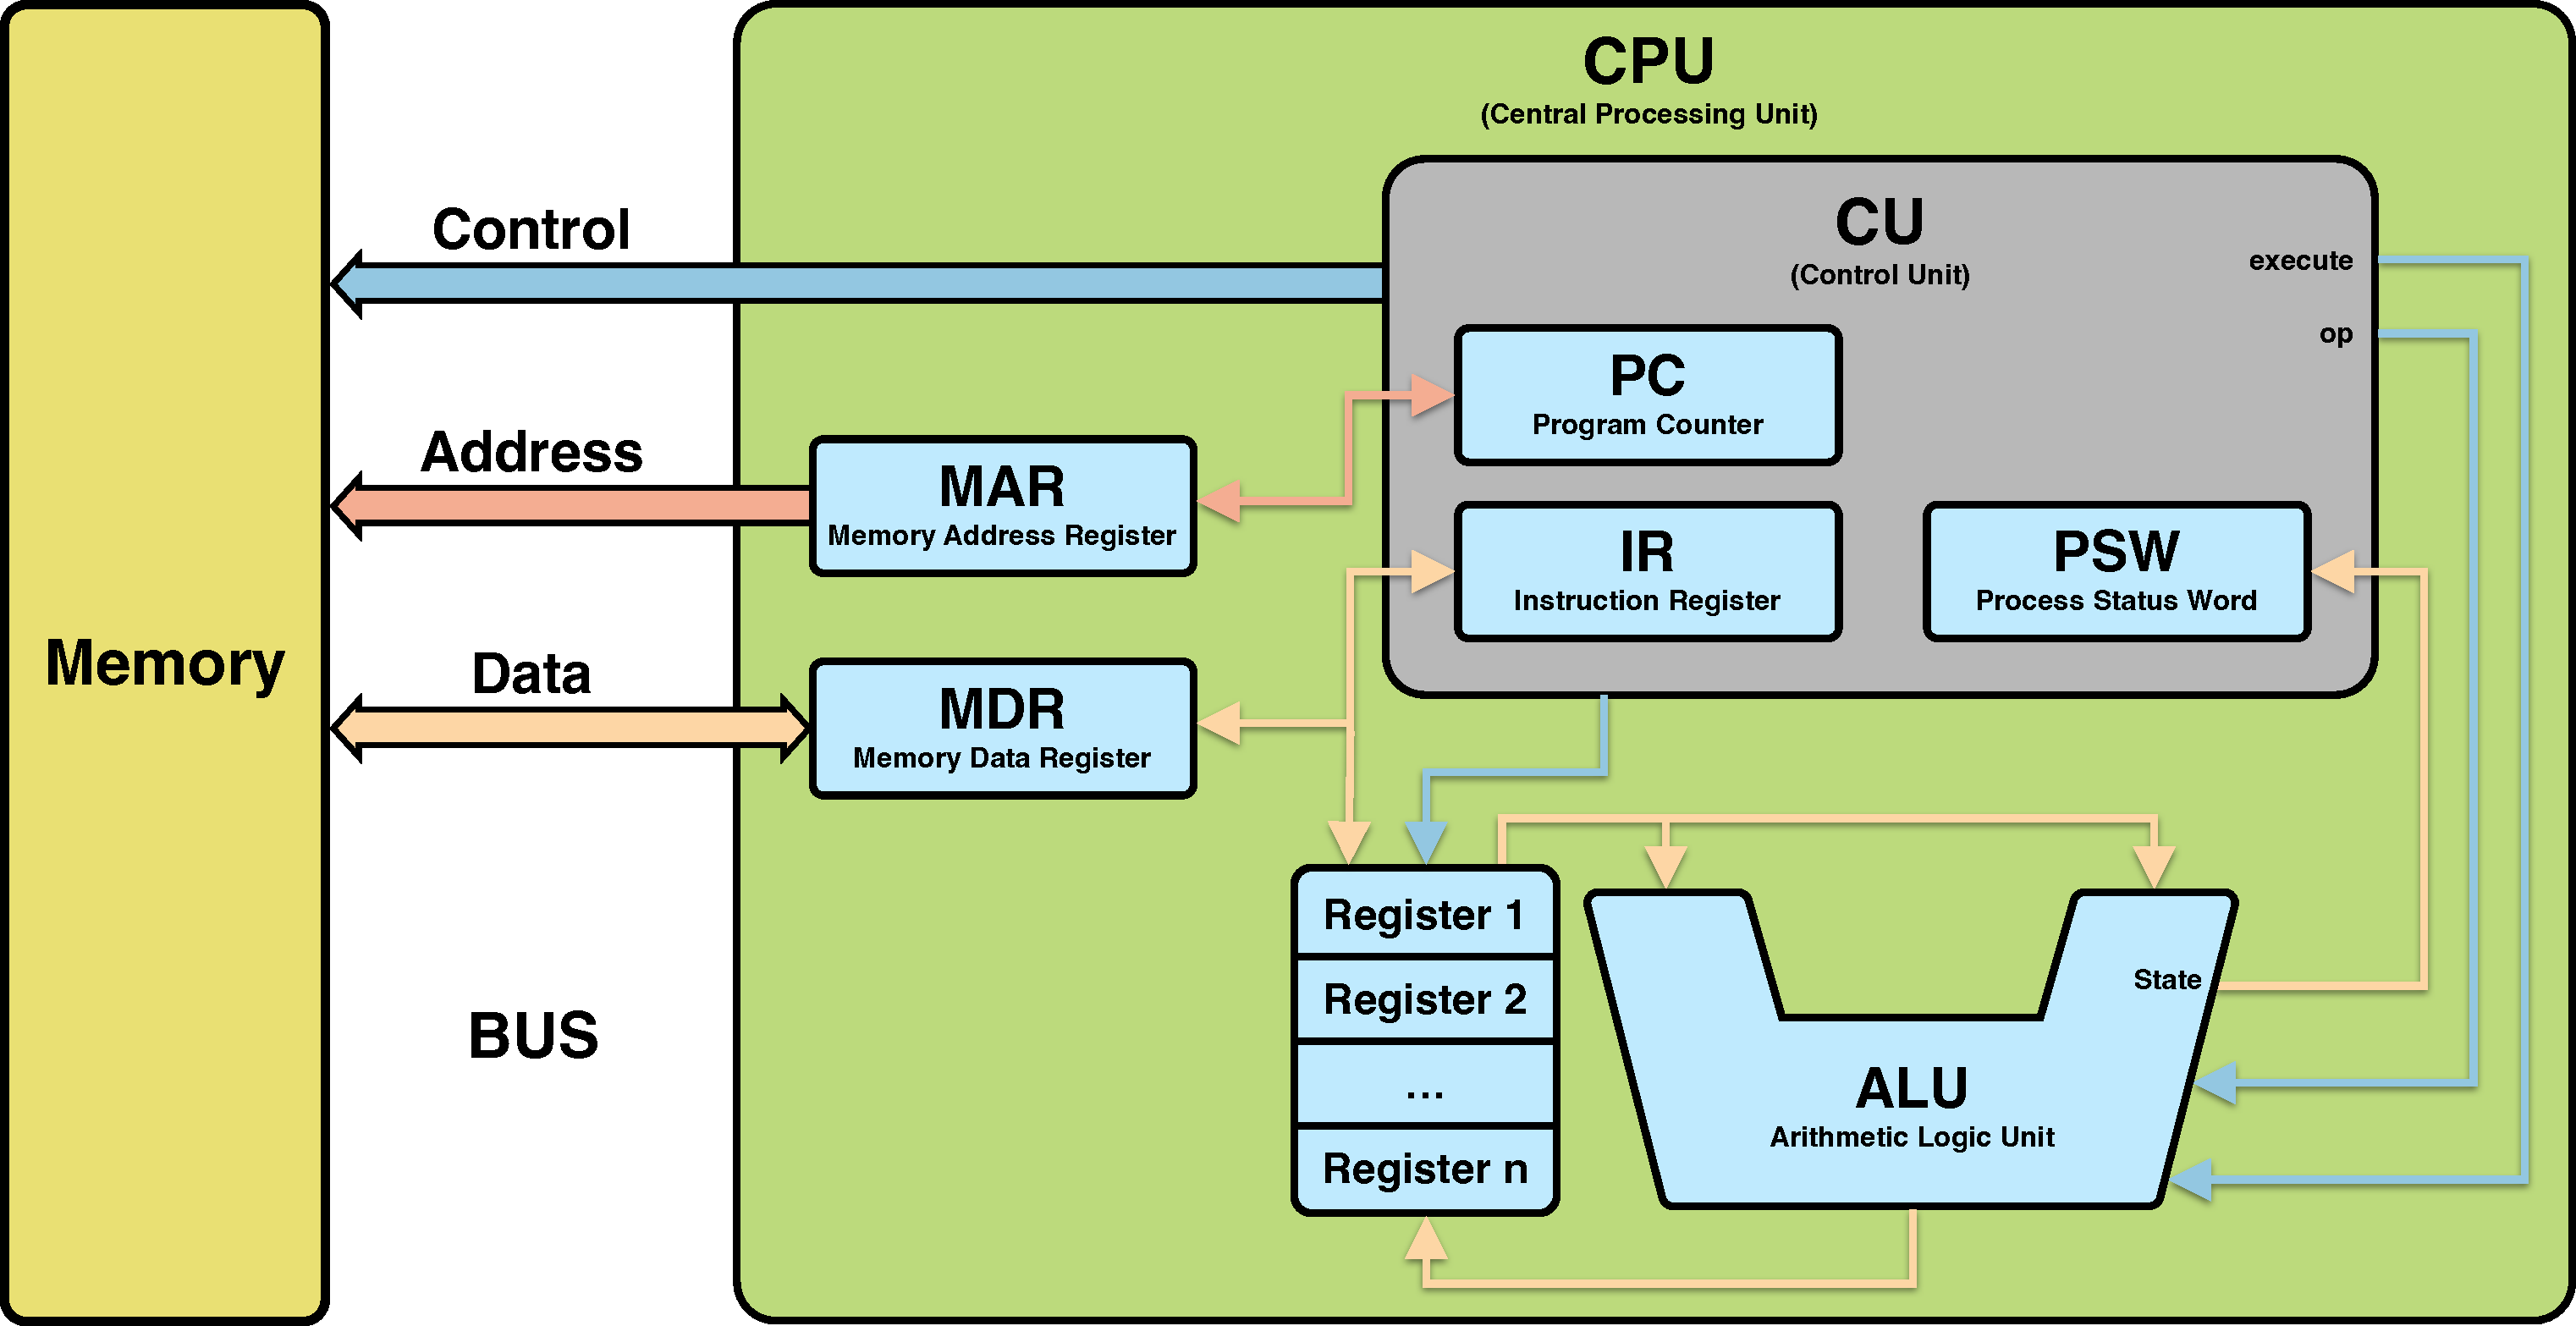
\includegraphics[width=0.7\linewidth]{images/4_cpu/architecture_cpu_complex.pdf}
%		\caption{La CPU: CU, ALU e registri}
		\label{fig:cpu_complex}
	\end{figure}
	
\end{frame}

